\documentclass[aip,twocolumn]{revtex4-2}
\usepackage{graphicx}
\usepackage{color}
\usepackage{amsmath,amssymb,bm}
\usepackage{physics}
\usepackage{siunitx}
\usepackage{hyperref}
\usepackage{xcolor}
\usepackage{mathtools}
\usepackage{enumitem}
%\setcounter{secnumdepth}{4}


%macros for math
\newcommand{\costh}{\ensuremath{\langle \cos^2 \theta_{\text{2D}} \rangle}}
\newcommand{\CSS}[0]{$\mathrm{CS_2}$}
\newcommand{\db}{\ensuremath{\Delta\beta}}
\newcommand{\dg}{\ensuremath{\Delta\gamma}}
\newcommand{\dt}{\ensuremath{\Delta t}}
\newcommand{\fcfg}{\ensuremath{f_{\mathrm{CFG}}}}
\newcommand{\fus}{\ensuremath{f_{\mathrm{us}}}}
\newcommand{\dfus}{\ensuremath{\Delta f_{\mathrm{us}}}}
\newcommand{\w}{\omega}
\newcommand{\wt}{\widetilde}
\newcommand{\ii}{\mathrm{i}}
\newcommand{\e}{\mathrm{e}}
\renewcommand{\dd}{\mathrm{d}}

%------------------------------------------------------------
\begin{document}

\title{Controlling Rotational Phase with an Optical Centrifuge}
%---------Authors---------
\author{Ian~MacPhail-Bartley}
\author{Gabriel Voith}
\author{S{\"o}ren Mahr}
\author{Cameron E. Peters}
\author{Valery Milner}
\email{vmilner@phas.ubc.ca}

\affiliation{$^{1}$Department of  Physics \& Astronomy, The University of British Columbia, Vancouver V6T-1Z1, Canada}

\date{\today}

\begin{abstract}
\textcolor{red}{Paper will be about: full TOD description of centrifuge, monitoring and/or stabilizing the phase, truncating usCFG,improving spectral resolution of cfCFG }

\end{abstract}

\maketitle
%====================================================================
%====================================================================

%====================================================================
\section{Introduction}
\label{sec:Introduction}
%----------Intro 1: What's a CFG ------------------------------------
In a series of two recent publications~\cite{Optical-centrifuge-with2025,An-ultraslow-optical-centrifuge2025}, we introduced two methods of creating an ``optical centrifuge''~\cite{Optical-Centrifuge-for-Molecules1999} based on the method of spectral focusing\textbf{[CITE SF paper]}.   \textcolor{red}{[Introduce centrifuge, applications, limitations..]}

%Needs more...

%----------Intro 3: field with TOD ------------
Up to third-order dispersion (TOD), a laser pulse can be described with instantaneous optical phase

\begin{equation}
    \label{Eq:phase}
\varphi(t) = \varphi_0 + \omega_0 t + \beta t^2 + \gamma t^3,
\end{equation}
\noindent where $\varphi_0$ and $\omega_0$ are the initial optical phase and optical carrier frequency, respectively, and $\beta$ and $\gamma$ are the linear chirp and TOD parameters, respectively. Generically, the two pulses comprising the optical centrifuge can be written with instantaneous optical frequencies 

\begin{equation}
\omega_\mathrm{u}(t) = \omega_0 + 2\beta_0 t + 3 \gamma_0 t^2 
\end{equation}
\noindent for the ``unshaped'' pulse and

\begin{align}
\omega_\mathrm{s}(t) &= \omega_0 + 2(\beta_0 + \db)(t + \dt) \\
&+ 3 (\gamma _0 + \dg)(t + \Delta t)^2 
\end{align}

\noindent for the ``shaped'' pulse. \dt{}, \db{}, and \dg{} represent the time delay, additional chirp rate, and additional TOD of the ``shaped'' pulse, with respect to the unshaped pulse's $\beta = \beta_0$ and $\gamma = \gamma_0$. Combining these two pulses,

\begin{align}
\label{Eq:CFG}
\begin{split}
\Omega (t) &= \frac{1}{2}[\omega_\mathrm{s}(t)  - \omega_\mathrm{u}(t) ]\\
&= \beta_0 \dt + \db t + \db \dt \\
&+ 3 \gamma_0 t \dt + \frac{3}{2} \gamma_0 (\dt)^2 \\
&+ \frac{3}{2} \dg t^2 + 3 \dg t \Delta t + \frac{3}{2} \dg (\dt)^2
\end{split}
\end{align}

\noindent is the centrifuge, fully accounting for third-order dispersion. The conventional optical centrifuge~\cite{Optical-Centrifuge-for-Molecules1999} operates in the regime of large \db{}, where only the second term in Eq.~\ref{Eq:CFG} is significant. In contrast, the ``constant frequency'' centrifuge~\cite{Optical-centrifuge-with2025} (cfCFG) operates with $\db, \dg \rightarrow 0$, and the baseline TOD from the laser source ($\gamma_0$) plays a significant role. For spectroscopic applications, any terms that vary with time throughout the pulse increase the effective line width of the centrifuge \textbf{[cite SF and NO Dimer]}. 

The intensity profile of an accelerating optical centrifuge  can play a similar role, if not all molecules follow its accelerated rotation to the end of the pulse. The intensity profile of the centrifuge field directly affects the projection of pendular states rotating \textit{with} the polarization vector onto the field-free molecular rotational states~\cite{Observation-of-nondispersing-classical-like2015}. Intuitively, a smooth falling edge results in molecules falling out of the centrifuge at different times, with different rotational frequencies i.e. populating a superposition of several different field-free states. Conversely, truncating the field abruptly can project molecules onto a single rotational state~\cite{Observation-of-nondispersing-classical-like2015}. 




%====================================================================
\section{Truncating the usCFG}
\label{sec:truncation}


%4f schematic 

%Reference Aleksey's paper with D2! Emphasize that shaping this way is not new, but include the technical details like using prisms because of the intensity at the focus, and picking longer lenses to avoid damage.

%====================================================================
\section{Real-Time Phase Tracking and Stabilization}
\label{sec:phase}

%----------Phase 1: How we can measure the phase with a spectrometer ------------
%Need to write out EXPLICITLY how this works, and why only *differences* between pulses show up.

%need optical schematic (Ian can make) 

%should highlight the limitation (frequency of oscillations WRT spectrometer resolution, how broader bandwidth lets you have higher frequencies with a lower resolution spectrometer)

%write out the fitting functions (expressions with real betas/gammmas etc.)

%----------Phase 2: Feedback loop with half wave plate ------------

%explain that this should be used for slower drift, while faster "jitter" requires phase tracking


%====================================================================
\section{Improving the Spectral Resolution of the cfCFG}
\label{sec:compensation}




%----------Characterization 1: Pileup -------------------------------
%Description of TOD contribution

\subsection{Compensating for TOD with a $4f$ pulse shaper}
%schematic of 4F pulse shaper
%good references to using an SLM to shape pulses, don't need to fully spell it out once more.

\begin{figure}
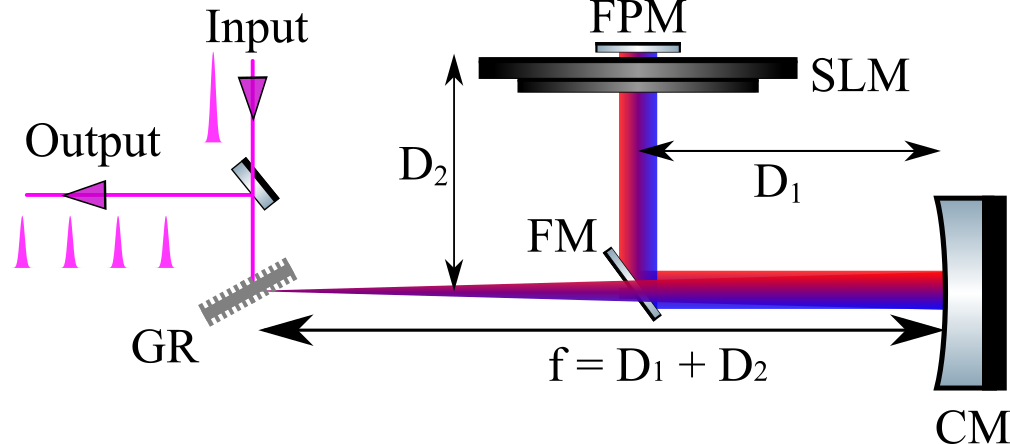
\includegraphics[width=\columnwidth]{figures/4f_folded.png}
\caption{\label{fig:4f_folded}\textcolor{red}{Will make more compact, and fix fonts. Show single chirped pulse in and out rather than the train... Should we include the Michelson afterwards? Might as well.}}
\end{figure}


%need to highlight benefits vs the method in the original spectral focusing paper, cons (energy limit from SLM)  


\subsection{Description of XCORR measurement}
%also clarify how once you've calibrated the spectrometer fit measurements this way, you can use it to directly read off the central frequency of the cfCFG and both frequency and acceleration of usCFG. 

\subsection{Demonstrating the improved resolution with Raman spectroscopy}
%mostly just need good references for how Raman works.

\begin{figure}
\includegraphics[width=\columnwidth]{figures/Raman_Setup.pdf}
\caption{\label{fig:raman_setup}\textcolor{red}{Will replace with correct font!}}
\end{figure}

%I think a single f_0 vs signal intensity scan for compensated vs uncompensated is sufficient, probably taken with oxygen at around 4x the centrifuge pulse duration? 
%Probably need 1/4 atmosphere or something to minimize collisional decoherence. 

%But the really best experiment would be showing that this makes lines resolvable with N2O, or something like that. (Since this allows for resolution greater than that of the mcpherson spectrometer!)

%====================================================================
\input{sections/conclusion}


%----------Acknowledgements -----------------------------------------
\begin{acknowledgments}
This research has been supported by grants from CFI, BCKDF, and NSERC, and carried out under the auspices of the UBC Centre for Research on Ultra-Cold Systems (CRUCS). The authors thank K. Wang for providing the initial schematics of the usCFG shaper. 
\end{acknowledgments}
%Create references using bibtex:
\bibliography{CFG_Shaping_Bibliography}

\end{document}
